\section{Lecture 1: Combinatorial Analysis}

\subsection{Counting}
\begin{frame}{Problem of Counting}
    \begin{example}
    \begin{itemize}
        \item  How many possible outcomes after rolling a die?
        \pause
   \item  How many possible outcomes after flipping a coin twenty times?\pause 
   ($2^{20}=1048576
$)
\pause
  \item   What is max number of different 6-place plates? Using capital letters and numbers only.\pause 
  ($36^6=2176782336$)
  \pause
  \item How many different birthday combinations in the class? Only consider the day and month? What if consider day month and year?
    \end{itemize}
    \end{example}
\end{frame}

\begin{frame}{}
    \bt[Basic principle of counting]
    For a sequence of finite experiments, denoted by $(r_1,r_2,\cdots, r_N)$, each experiment $r_j$ can output $n_j$ results, then the total number of outputs is 
\begin{align}
\label{eq:prin of counting}
\prod_{j=1}^Nn_j:=n_1n_2\cdots n_N.
\end{align}
    \et
\end{frame}
\subsection{Permutation}
\begin{frame}{Permutation}
    \begin{itemize}
        \item Given an object of $n$ elements, an arrangement is called a permutation.
        \item For example, flipping coin twice, possible permutations are: HH,HT,TH,TT
        \item A sequence of letters $(a,b,c)$, there are 6 permutations: $$abc,acb,bac,bca,cab,cba.$$
    \end{itemize}
    \begin{block}{Questions}
    How many permutations for the sequence $\{a,a,b,c,c,d\}$? 
    \end{block}

\end{frame}
\begin{frame}{Permutation}
\bt[Basic permutation theorem]
\label{permuation theorem}
Suppose there are $n$ distinct objects, then the number of total permutations is 
\begin{align}
    n!:=n(n-1)(n-2)\cdots 2\cdot 1.
\end{align}
\et
\bt[General permutation theorem]
\label{gen permuation thm}
Suppose there $n$ objects with $n_1$ are alike, $n_2$ are alike,..., $n_r$ are alike, where $n_1+n_2+...+n_r=n$, then the total number of permutations are 
\begin{align}
    \frac{n!}{n_1!n_2!\cdots n_r!}
\end{align}
\et
    
\end{frame}
\begin{frame}{Permutation Model}
	\begin{itemize}
		\item Assign $n$ hats to $k$ people, how many ways?\pause
		\item If all hats are different, there are two cases: case 1, $k>n$, we will back to this later; case 2, $k\leq n$, then there are $n(n-1)\cdots (n-k+1)=\frac{n!}{k!}$ ways.
		\pause
		\item If there are $n_1$ white hats and $n_2$ black, suppose $n_1+n_2=n\geq k\geq \max\{n_1,n_2\}\}$, how many ways?
		\pause
		\item \red{A little bit hard.}  Symbolically, we have
		\[\sum_{k_1+k_2=k,k_1\leq n_1,k_2\leq n_2}\frac{n_1!n_2!}{k_1!k_2!}\]
	\end{itemize}
\end{frame}

\subsection{Combination}
\begin{frame}{Combination}
A \textit{combination} is a process by selecting objects from a given object. For example:
\begin{itemize}
    \item Consider the set $\{A,B,C,D\}$, how many different way of selecting 2 letters from the set? It's not hard to write down all possible combinations. They are $AB,AC,AD,BC,BD,CD$.
    \item \red{The order doesn't matter in dealing with combinations.}
    \item \blue{Question:} How to count the number of possible combinations in general, say, select $m$ items from $n$ \textbf{distinct} objects?
    \item Use the basic principle of counting!
\end{itemize}
    
\end{frame}

\begin{frame}{Combination}
Here is the reasoning. Suppose you have a set of $n$ distinct objects, you want to choose $m$ distinct objects from there. The first time, you have $n$ choices. The second time you will have $n-1$ choices. And the $m$-th time you only have $n-m+1$ choices. Then we can apply \red{ the basic principle of counting} to conclude that total number of (ordered) choices is 
\begin{align*}
    n(n-1)\cdots (n-m+1)=\frac{n!}{(n-m)!}.
\end{align*}
But, since we don't care the order of the outcomes, it follows the number of different way of picking $m$ objects is
\begin{align*}
    \frac{n!}{m!(n-m)!}.
\end{align*}
    
\end{frame}

\begin{frame}{Hat problem}
	\begin{itemize}
		\item Back to the hat problem, now let us consider $n< k$ case.
		\item First we need select $k-n$ people from the $k$ people group, that's \red{stage one}.
		\item \red{Stage two} is assign the $n$ hats to the rest $n$ people.
		\item Using the basic counting principal, we have
		\[\binom{k}{k-n}n!=\frac{k!}{(k-n)!}\]
	\end{itemize}
\end{frame}

\begin{frame}{Combination}
A notation will be introduced to denote the number of combination:
\[
\binom{n}{m}:=\frac{n!}{m!(n-m)!}.
\]
Using this notation, we can state a useful algebra theorem
\bt [The Binomial theorem]
$$
    (x+y)^n=\sum_{k=0}^n\binom{n}{k}x^ky^{n-k}.
$$
\et 
\bc By choosing $x=y=1$, we get 
$$
    2^n=\sum_{k=0}^n\binom{n}{ k}.
$$
\ec
\end{frame}

\begin{frame}{A combinatorial proof}
\begin{proof}
    Let's consider two sets $\{x_1,\cdots,x_n\}$and $\{y_1,\cdots,y_n\}$, consider the following product
    \[(x_1+y_1)(x_2+y_2)\cdots(x_n+y_n).\]
    To expand this product, we basically select a factor from each bracket, and the factor is of the form
    $
        z_1z_2\cdots z_n,
$
    where $z$ could be $x$ or $x$. Each factor represents a way of selecting objects. Since the order doesn't matter, the number of way of selecting $k$ $x$ and $n-k$ $y$ is given by $\binom{n}{k}$. Now, let all $x_i=x$ and $y_i=y$, we get
    \begin{align*}
        (x+y)^n=\sum_{k=0}^n\binom{n}{k}x^ky^{n-k}.
    \end{align*}
\end{proof}
    
\end{frame}

\begin{frame}{A remark}
	\textbf{Remark:} Combination doesn't feel the order, thus needs to divide by permutations. To get rid of labels is equivalent to eliminating the order, thus, we can consider
	\[\binom{n}{m}=\frac{n!}{m!(n-m)!}\]
	as selecting $m$ $x$ and $n-m$ $y$ and then divide by their permutations $m!$ and $(n-m)!$ respectively. And this can be generalized to multi-variables.
\end{frame}

\begin{frame}{Combination}
    \bt[The multinomial theorem]
\label{multinomial thm}
\begin{align}
    \le(\sum_{k=1}^rx_k\ri)^n=\sum_{n_1+n_2+\cdots+n_r=n}\binom{n}{ n_1,n_2,...,n_r}x_1^{n_1}x_2^{n_2}\cdots x_r^{n_r}.
\end{align}
The sum on the right hand side is over all non-negative integer valued vectors $(n_1,...,n_r)$ such that $\sum_{k=1}^rn_k=n$. 
\et

\textbf{Question:} Find the Taylor expansion formula for multi-variable functions and understand the meaning of the Taylor coefficients. Write down the Taylor expansion (near origin) for the following functions:
\begin{align*}
    e^{x+y},\quad \sin(x+y),\quad \ln(x^2+y^2+1).
\end{align*}
\end{frame}
\subsection{Practice}
\begin{frame}{Practice Problems}
\begin{itemize}
    \item How many 5-card poker hands are there? No jokers.
    \pause
    \item If 8 identical apples are to be divided among 4 students, how many divisions are possible? What if each student must at least receive one?
    
    \item How many non-negative integer solutions of the following equation: $x+y+z=100$?
   
    \item Number of non-negative solutions to the following inequality:
    \[\sum_{i=1}^n x_i\leq k?\]\pause
     \item Show $\sum_{k=1}^n k\binom{n}{k}=n\cdot 2^{n-1}.$
    \item Show $\sum_{k=1}^n k^2\binom{n}{k}=n(n+1)\cdot 2^{n-2}.$
\end{itemize}
    
\end{frame}

\begin{frame}{More Problems}

\begin{columns}
\begin{column}{0.5\textwidth}
\begin{figure}[ht]
    \centering
    
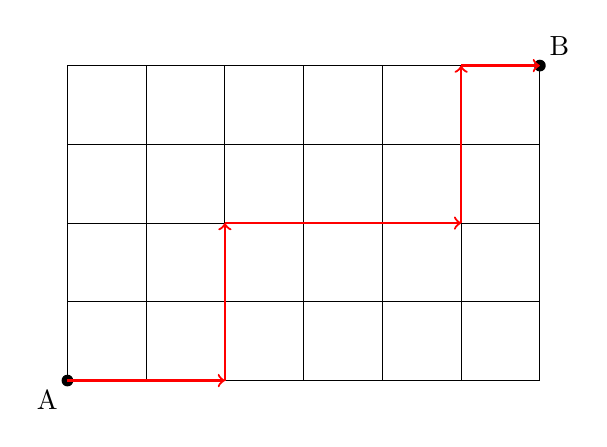
\begin{tikzpicture}
\draw (0,0) node[anchor=north east]{A} grid (6,4) node[anchor=south west]{B};
 \node at (0,0) [circle,fill,inner sep=1.5pt]{};
 \node at (6,4) [circle,fill,inner sep=1.5pt]{};
 \draw[thick,->,red] (0,0) -- (2,0);
 \draw[thick,->,red] (2,0) -- (2,2);
 \draw[thick,->,red] (2,2) -- (5,2);
 \draw[thick,->,red] (5,2) -- (5,4);
 \draw[thick,->,red] (5,4) -- (6,4);
\end{tikzpicture}

    \caption{An exmaple path from A to B.}
    \label{fig: Counting path}
\end{figure}
\end{column}
\begin{column}{0.5\textwidth}
\textbf{Question:} A bug is walking from A to B, and it can only move up or right, the figure shows a possible path from A to B. How many possible different ways from A to B? The coordinate of A and B are $(0,0)$ and $(6,4)$ respectively. \red{How to generalize it to arbitrary two points? What if the bug must pass a provided point, say $(2,2)$, how many ways it can possible go from A to B? }
\end{column}
\end{columns}
\end{frame}
\subsection{Summary}
\begin{frame}{Summary}
\begin{enumerate}
    \item If the elements are \textbf{reusable}, then \textbf{Basic principal of counting}; Else
    \item If there are $n$ distinct objects, then \textbf{Permutation}; Else
    \item if there are repeating objects, then \textbf{General permutation}; Else
    \item if \textbf{Order} doesn't matter, then standard \textbf{combination}; Else
    \item Combination \textbf{times} permutation.
\end{enumerate}
    
\end{frame}

\subsection{Homework}
\begin{frame}{Homework 1 }
	\begin{columns}
		\begin{column}{0.5\textwidth}
			\begin{itemize}
				\item Ross Chapter I Problems: 3, 15, 19, 31
				\item Ross Chapter I Theoretical Exercises: 11, 12, 14 
				\item Given a pack of 52 standard cards, selecting 5 cards, how many ways to get a pair? What about three of a kind?
				\item Simplify $\sum_{k=1}^n k^3\binom{n}{k}$, and prove it. 
			\end{itemize}
		\end{column}
	\begin{column}{0.5\textwidth}
		\begin{itemize}
			
			\item (Whole line 1D Random Walk) Consider a particle is moving on the real integer line ($\cdots,-3,-2,-1,0,1,2,3,\cdots$), starting at 0, each step it can move left/right one unit, after 10 moves, how many different paths can happen? 
			\item (Half line 1D Random Walk) Now consider starting point at 0, and the domain is now $\Z_+\cup \{0\}=\{0,1,2,3,\cdots\}$, how many paths of length 10?
			\item For the half line 1D RW, what if the starting point is $x\in \Z_+$, how many paths of length 10?
		\end{itemize}
	\end{column}
	\end{columns}
\end{frame}
